\documentclass[12pt]{article}

\usepackage[spanish]{babel}
\usepackage{hyperref}
\usepackage{graphicx}
\usepackage{listings}
\usepackage{color}
\usepackage{multicol}
\usepackage{amssymb}
\usepackage{enumitem}
\usepackage{here}
\usepackage{dsfont}
\usepackage{amsmath}
\usepackage{tipa}
\spanishdecimal{.}

\title{Matemáticas para las Ciencias Aplicadas I}
\title{
	Segunda Lista de Problemas \\
	\textbf{Tercera  Parte} \\
	\vspace{1ex}
	\large Matemáticas para las Ciencias Aplicadas I \\
	Facultad de Ciencias, UNAM}

\date{\today}

\author{Flores Morán Julieta Melina \\ Zarco Romero José Antonio}

\begin{document}

\maketitle

%% 11, 28, 31 y 41
%% 25, 31 y 40

%% 1
\section{Ejercicio 11} name \\

\begin{figure}[h!]
\centering
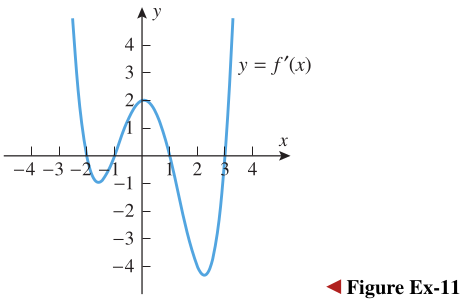
\includegraphics[width=0.5\textwidth]{../img/img_Lista2/3_11.png}
\end{figure}
La figura adjunta muestra la gráfica de $y = f'(x)$ para una función $f$ no especificada.
\begin{enumerate}[label=(\alph*)]
\item ¿Para qué valores de $x$ la curva $y = f(x)$ tiene una recta tangente horizontal?
\item ¿En qué intervalos la curva $y = f(x)$ tiene rectas tangentes con pendiente positiva?
\item ¿En qué intervalos la curva $y = f(x)$ tiene rectas tangentes con pendiente negativa?
\item Dado que $g(x) = f(x) \sin x$, encuentre $g''(0)$.
\end{enumerate}

%% 2
\section{Ejercicio 28} name \\

En cada parte, evalúa la expresión dado que $f(1)=1$, $g(1)=-2$, $f'(1)=3$ y $g'(1)=-1$.
\begin{enumerate}[label=(\alph*)]
\item $\frac{d}{dx} \lbrack f(x)g(x) \rbrack |_{x=1}$
  \begin{equation*}
    \begin{split}
      \frac{d}{dx} \lbrack f(x)g(x) \rbrack |_{x=1}
      & = f(x)g'(x)+g(x)f'(x) |_{x=1} \\
      & = f(1)g'(1)+g(1)f'(1) \\
      & = (1 \cdot -1) + (-2 \cdot 3) \\
      & = -1 + (-6) \\
      & = -1-6 \\
      & =-7
    \end{split}
  \end{equation*}

\item $\frac{d}{dx} \lbrack \frac{f(x)}{g(x)} \rbrack |_{x=1}$
  \begin{equation*}
    \begin{split}
      \frac{d}{dx} \lbrack \frac{f(x)}{g(x)} \rbrack |_{x=1}
      & = \frac{g(x)f'(x)-f(x)g'(x)}{\lbrack g(x) \rbrack ^2} |_{x=1} \\
      & = \frac{g(1)f'(1)-f(1)g'(1)}{\lbrack g(1) \rbrack ^2}\\
      & = \frac{(-2 \cdot 3)-(1 \cdot -1)}{(-2) ^2}\\
      & = \frac{(-6)-(-1)}{4}\\
      & = \frac{-6+1}{4}\\
      & = - \frac{5}{4}
    \end{split}
  \end{equation*}

\item $\frac{d}{dx} \lbrack \sqrt{f(x)} \rbrack |_{x=1}$
  \begin{equation*}
    \begin{split}
      \frac{d}{dx} \lbrack \sqrt{f(x)} \rbrack |_{x=1}
      & = \frac{d}{dx} { [f(x)]^{\frac{1}{2}} } |_{x=1} \\
      & = \frac{1}{2}[f(x)]^{-\frac{1}{2}} \cdot f'(x) |_{x=1} \\
      & = \frac{1}{2}[f(1)]^{-\frac{1}{2}} \cdot f'(1)  \\
      & = \frac{1}{2}(1)^{-\frac{1}{2}} \cdot 3  \\
      & = \frac{1}{2}(1) \cdot 3  \\
      & = \frac{3}{2}
    \end{split}
  \end{equation*}

\item $\frac{d}{dx} \lbrack f(1)g'(1) \rbrack$
  \begin{equation*}
    \begin{split}
      \frac{d}{dx} \lbrack f(1)g'(1) \rbrack
      & = \frac{d}{dx} \lbrack 1 \cdot -1 \rbrack \\
      & = \frac{d}{dx} \lbrack -1 \rbrack \\
      & = 0
    \end{split}
  \end{equation*}
  
\end{enumerate}

%% 3
\section{Ejercicio 31} name \\

Encuentre $f'(x)$.
\begin{enumerate}[label=(\alph*)]
\item .
\end{enumerate}

%% 4
\section{Ejercicio 41} name \\

Supongamos que $f'(x) = 2x \cdot f(x)$ y $f(2) = 5$.
\begin{enumerate}[label=(\alph*)]
\item .
\end{enumerate}

%% 5
\section{Ejercicio 25} name \\

Utilice la diferenciación implícita para encontrar la pendiente de la recta tangente a la curva en el punto especificado y verifique que su respuesta sea consistente con la gráfica adjunta en la página siguiente.
\begin{figure}[h!]
\centering
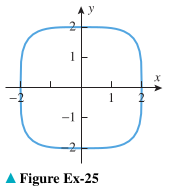
\includegraphics[width=0.5\textwidth]{../img/img_Lista2/3_25.png}
\end{figure}

%% 6
\section{Ejercicio 31} name \\

Utilice la diferenciación implícita para encontrar la derivada especificada.
\[ a^2 \omega^2 + b^2 \lambda^2 = 1 \text{ (a, b constantes); } d\omega /d\lambda \]

%% 7
\section{Ejercicio 40} name \\

Se dice que dos curvas son \textbf{ortogonales} si sus rectas tangentes son perpendiculares en cada punto de intersección, y se dice que dos familias de curvas son \textbf{trayectorias ortogonales} entre sí si cada miembro de una familia es ortogonal a cada miembro de la otra familia. Esta terminología se utiliza en estos ejercicios.
%%La figura adjunta muestra algunos miembros típicos de las familias de hipérbolas $xy=c$ (curvas negras) y $x^2 − y^2 = k$ (curvas grises), donde $c \neq 0$ y $k \neq 0$. Utilice la sugerencia del ejercicio 39 para demostrar que estas familias son trayectorias ortogonales entre sí. [\textit{Sugerencia}: para que las rectas tangentes sean perpendiculares en un punto de intersección, las pendientes de esas rectas tangentes deben ser recíprocas negativas entre sí.]
\begin{figure}[h!]
\centering
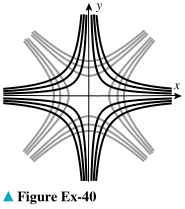
\includegraphics[width=0.5\textwidth]{../img/img_Lista2/3_40.png}
\end{figure}

\end{document}
